\documentclass{beamer}
\usepackage[utf8]{inputenc}
\usepackage{listings}
\usepackage{xcolor}
\usepackage{hyperref}
\usepackage{tikz}
\usetikzlibrary{shapes.geometric, arrows.meta, positioning}

\usetheme{Madrid}
\hypersetup{breaklinks=true}

% Python code style
\definecolor{codegray}{rgb}{0.95,0.95,0.95}
\definecolor{keyword}{rgb}{0.0,0.0,0.6}
\definecolor{comment}{rgb}{0.0,0.5,0.0}
\definecolor{string}{rgb}{0.64,0.08,0.08}
\definecolor{labcolor}{rgb}{0.1,0.4,0.1}

\lstdefinestyle{codeStyle}{
    language=Python,
    backgroundcolor=\color{codegray},
    commentstyle=\color{comment}\itshape,
    keywordstyle=\color{keyword}\bfseries,
    stringstyle=\color{string},
    basicstyle=\ttfamily\footnotesize,
    breaklines=true,
    frame=single,
    showstringspaces=false,
    tabsize=4,
    morekeywords={self, True, False, None, with, as, match, case}
}

% TikZ styles for flowcharts
\tikzset{
    startstop/.style={rectangle, rounded corners, draw, fill=blue!20, minimum width=2cm, minimum height=0.6cm},
    decision/.style={diamond, draw, fill=yellow!20, aspect=2, minimum width=1.5cm},
    process/.style={rectangle, draw, fill=green!10, minimum width=2cm, minimum height=0.6cm},
    arrow/.style={-{Stealth}, thick}
}

\title{Python for Cheminformatics \& Bioinformatics}
\subtitle{Combined Lessons \& Labs}
\author{Nirajan Bhattarai}
\institute{AI-Driven Drug Development Training}
\date{February 2026}

\begin{document}

% ============================================
% TITLE SLIDE
% ============================================
\begin{frame}
    \titlepage
\end{frame}

% ============================================
% OVERVIEW
% ============================================
\begin{frame}{Course Overview}
    \tableofcontents
\end{frame}

\begin{frame}{Learning Objectives}
    \footnotesize
    \textbf{By the end of this course, you will be able to:}
    \vspace{0.3em}
    \begin{enumerate}
        \item Write Python code for basic data manipulation
        \item Work with molecular data (SMILES, formulas, properties)
        \item Process biological sequences (DNA, RNA, protein)
        \item Use control flow (conditionals, loops) for data filtering
        \item Organize data using lists, dictionaries, and sets
        \item Create reusable functions for cheminformatics tasks
        \item Read/write files (CSV, FASTA, JSON)
        \item Use NumPy arrays and Pandas DataFrames
        \item Apply concepts to Rosalind bioinformatics problems
    \end{enumerate}
\end{frame}

\begin{frame}{Prerequisites \& Setup}
    \small
    \textbf{Prerequisites:}
    \begin{itemize}
        \item Basic computer literacy
        \item No prior programming experience required
        \item Interest in drug discovery / life sciences
    \end{itemize}
    \vspace{0.5em}
    \textbf{Software Setup:}
    \begin{itemize}
        \item Python 3.8+ installed
        \item IDE: VS Code, PyCharm, or Jupyter Notebook
        \item Libraries: \texttt{pip install numpy pandas rdkit}
    \end{itemize}
    \vspace{0.5em}
    \textbf{Resources:}
    \begin{itemize}
        \item Rosalind.info -- Bioinformatics problems
        \item ChEMBL -- Bioactivity database
        \item PubChem -- Chemical information
    \end{itemize}
\end{frame}

% ============================================
% PREREQUISITE: DATA TYPES IN DRUG DISCOVERY
% ============================================
\section{Data Types in Drug Discovery}

\begin{frame}{Data Types You'll Encounter}
    \small
    \textbf{Before we start coding, let's understand the data types used in drug discovery:}
    \vspace{0.5em}
    \begin{columns}[T]
        \begin{column}{0.48\textwidth}
            \textbf{Cheminformatics:}
            \begin{itemize}
                \item SMILES -- Molecular structures
                \item Molecular Descriptors (MW, LogP)
                \item Activity Data (IC50, pIC50)
                \item Lipinski Properties
            \end{itemize}
        \end{column}
        \begin{column}{0.48\textwidth}
            \textbf{Bioinformatics:}
            \begin{itemize}
                \item DNA Sequences (A, T, G, C)
                \item RNA Sequences (A, U, G, C)
                \item Protein Sequences (amino acids)
                \item FASTA Format
            \end{itemize}
        \end{column}
    \end{columns}
    \vspace{0.5em}
    \textit{Understanding these data types is essential for the exercises in this course.}
\end{frame}

\begin{frame}{SMILES: Simplified Molecular Input Line Entry System}
    \small
    \textbf{What is SMILES?}\\
    A text-based notation for representing chemical structures as strings.
    \vspace{0.5em}
    
    \textbf{Key Rules:}
    \begin{itemize}
        \item Atoms: C, N, O, S, P, F, Cl, Br, I (organic subset)
        \item Bonds: single (default), double (=), triple (\#), aromatic (:)
        \item Rings: Numbers indicate ring closures (e.g., \texttt{c1ccccc1} = benzene)
        \item Branches: Parentheses for side chains (e.g., \texttt{CC(C)C} = isobutane)
    \end{itemize}
    \vspace{0.3em}
    
    \textbf{Examples:}
    \begin{tabular}{ll}
        \texttt{CCO} & Ethanol \\
        \texttt{CC(=O)O} & Acetic acid \\
        \texttt{c1ccccc1} & Benzene \\
        \texttt{CC(=O)Oc1ccccc1C(=O)O} & Aspirin \\
    \end{tabular}
\end{frame}

\begin{frame}{Molecular Descriptors \& Activity Data}
    \small
    \textbf{Key Molecular Properties:}
    \begin{tabular}{lll}
        \textbf{Property} & \textbf{Description} & \textbf{Typical Range} \\
        \hline
        MW & Molecular Weight (Da) & 150--500 Da \\
        LogP & Lipophilicity & -2 to 5 \\
        HBD & H-bond Donors & 0--5 \\
        HBA & H-bond Acceptors & 0--10 \\
    \end{tabular}
    \vspace{0.5em}
    
    \textbf{pIC50 Conversion:}
    \begin{equation*}
        \text{pIC50} = -\log_{10}(\text{IC50}_{\text{M}}) = 9 - \log_{10}(\text{IC50}_{\text{nM}})
    \end{equation*}
    
    \textbf{Activity Classification:}
    \begin{tabular}{lll}
        pIC50 $\geq$ 8 & IC50 $\leq$ 10 nM & Highly Active \\
        6--8 & 10--1000 nM & Active \\
        $<$ 6 & $>$ 1000 nM & Inactive \\
    \end{tabular}
\end{frame}

\begin{frame}{DNA, RNA \& Protein Sequences}
    \small
    \textbf{DNA:} A, T, G, C (double helix, base pairing: A-T, G-C)\\
    \textbf{RNA:} A, U, G, C (single strand, T $\to$ U)\\
    \textbf{Protein:} 20 amino acids encoded by codons
    \vspace{0.5em}
    
    \begin{center}
        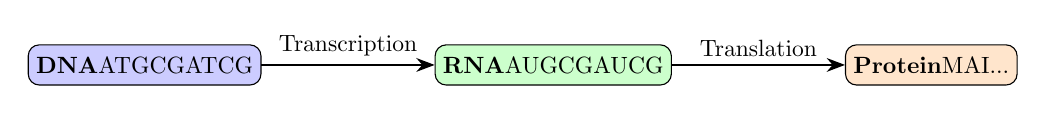
\begin{tikzpicture}[node distance=2.2cm, scale=0.85, every node/.style={scale=0.85}]
            \node (dna) [startstop, fill=blue!20, minimum width=2.5cm] {\textbf{DNA}\\ATGCGATCG};
            \node (rna) [startstop, fill=green!20, right=of dna, minimum width=2.5cm] {\textbf{RNA}\\AUGCGAUCG};
            \node (protein) [startstop, fill=orange!20, right=of rna, minimum width=2.5cm] {\textbf{Protein}\\MAI...};
            
            \draw[arrow] (dna) -- node[above] {Transcription} (rna);
            \draw[arrow] (rna) -- node[above] {Translation} (protein);
        \end{tikzpicture}
    \end{center}
    \vspace{0.3em}
    
    \textbf{Key Operations:}
    \begin{itemize}
        \item Transcribe: DNA $\to$ RNA (replace T with U)
        \item Reverse Complement: A$\leftrightarrow$T, G$\leftrightarrow$C, then reverse
        \item GC Content: (G + C) / total $\times$ 100\%
    \end{itemize}
\end{frame}

% ============================================
% SECTION 1: PYTHON BASICS
% ============================================
\section{Python Basics (Lessons 1--6B)}

% ============================================
% LESSON 1: VARIABLES & DATA TYPES
% ============================================
\subsection{Lesson 1: Variables \& Data Types}

\begin{frame}{Lesson 1: Learning Objectives}
    \small
    \textbf{Learning Objectives:}
    \begin{itemize}
        \item Understand how variables store data in memory
        \item Identify Python's core data types (int, float, str, bool)
        \item Perform type conversions between data types
    \end{itemize}
    \vspace{0.5em}
    \textbf{Applications:}
    \begin{itemize}
        \item Store compound properties (MW, LogP, SMILES)
        \item Represent bioactivity measurements (IC50, pIC50)
        \item Handle DNA/RNA sequence data
    \end{itemize}
\end{frame}

\begin{frame}{Lesson 1: Variables \& Data Types}
    \small
    \textbf{Concept:} Variables store data in memory.\\[0.5em]
    Python data types: \texttt{int}, \texttt{float}, \texttt{str}, \texttt{bool}, \texttt{NoneType}\\[0.5em]
    \textbf{Type Conversion:} \texttt{int()}, \texttt{float()}, \texttt{str()}, \texttt{bool()}\\[0.5em]
    \textbf{Drug Discovery Scenarios:}
    \begin{itemize}
        \item Compound Info (name, MW, LogP, SMILES)
        \item Bioactivity Data (IC50, Ki, pIC50)
        \item DNA/RNA Sequences (nucleotide strings)
    \end{itemize}
\end{frame}

\begin{frame}[fragile]{Lesson 1 Code Example}
    \small
    \begin{lstlisting}[style=codeStyle]
# Compound Info
compound_name = "Aspirin"
mw = 180.16  # Molecular Weight (Da)
logP = 1.19  # Lipophilicity
smiles = "CC(=O)OC1=CC=CC=C1C(=O)O"

# Bioactivity Data
ic50_nM = 5.2  # IC50 in nanomolar
pic50 = 8.28   # -log10(IC50 in M)
is_active = True

# DNA Sequence
dna_seq = "ATGCGATCGATCG"
seq_length = len(dna_seq)

# Type Conversion
ic50_str = str(ic50_nM)
mw_int = int(mw)

print(f"{compound_name}: MW={mw}, pIC50={pic50}")
    \end{lstlisting}
\end{frame}

% --- LAB 1 ---
\begin{frame}{\textcolor{labcolor}{Lab 1: Variables \& Data Types}}
    \footnotesize
    \textbf{Objective:} Practice storing and converting molecular and sequence data.
    \vspace{0.3em}
    \begin{block}{Exercise 1.1 -- Compound Data Storage}
        Create variables for a drug compound:
        \begin{itemize}\setlength{\itemsep}{0pt}
            \item Name (string): ``Ibuprofen''
            \item SMILES (string): ``CC(C)CC1=CC=C(C=C1)C(C)C(=O)O''
            \item Molecular weight (float): 206.28
            \item pIC50 (float): 6.1
            \item Is active (bool): True if pIC50 $\geq$ 6.0
        \end{itemize}
        Print all values using f-strings.
    \end{block}
\end{frame}

\begin{frame}{\textcolor{labcolor}{Lab 1: Variables \& Data Types (cont.)}}
    \small
    \begin{block}{Exercise 1.2 -- DNA Sequence}
        Store a DNA sequence: ``ATGCGATCGATCGATCGATCG''\\
        Calculate and print:
        \begin{itemize}
            \item Sequence length
            \item Number of adenines (A)
            \item Number of thymines (T)
        \end{itemize}
    \end{block}
    \vspace{0.5em}
    \begin{block}{Exercise 1.3 -- Type Conversion}
        Given IC50 = ``5.2'' (string), convert to float and calculate pIC50.\\
        Store the result as both float and formatted string (2 decimals).
    \end{block}
\end{frame}

% ============================================
% LESSON 2: OPERATORS
% ============================================
\subsection{Lesson 2: Operators}

\begin{frame}{Lesson 2: Learning Objectives}
    \small
    \textbf{Learning Objectives:}
    \begin{itemize}
        \item Use arithmetic operators for scientific calculations
        \item Apply comparison operators to filter data
        \item Combine conditions using logical operators
    \end{itemize}
    \vspace{0.5em}
    \textbf{Applications:}
    \begin{itemize}
        \item Convert IC50 to pIC50 ($-\log_{10}$)
        \item Check Lipinski Rule of Five compliance
        \item Calculate GC content in DNA sequences
    \end{itemize}
\end{frame}

\begin{frame}{Lesson 2: Operators}
    \small
    \textbf{Arithmetic:} \texttt{+}, \texttt{-}, \texttt{*}, \texttt{/}, \texttt{\%}, \texttt{**}\\[0.5em]
    \textbf{Comparison:} \texttt{>}, \texttt{<}, \texttt{==}, \texttt{!=}, \texttt{>=}, \texttt{<=}\\[0.5em]
    \textbf{Logical:} \texttt{and}, \texttt{or}, \texttt{not}\\[0.5em]
    \textbf{Drug Discovery scenarios:} Calculate pIC50, check Lipinski rules, filter active compounds
\end{frame}

\begin{frame}[fragile]{Lesson 2 Code Example}
    \small
    \begin{lstlisting}[style=codeStyle]
import math

# IC50 to pIC50 conversion
ic50_nM = 10.0  # nanomolar
ic50_M = ic50_nM * 1e-9  # convert to molar
pic50 = -math.log10(ic50_M)  # pIC50 = 8.0
print(f"IC50: {ic50_nM} nM -> pIC50: {pic50:.2f}")

# Lipinski Rule of Five checks
mw, logP, hbd, hba = 450, 3.5, 2, 6
lipinski_ok = (mw <= 500) and (logP <= 5) and (hbd <= 5) and (hba <= 10)
print(f"Passes Lipinski: {lipinski_ok}")

# GC Content calculation
seq = "ATGCGCGCTA"
gc_count = seq.count("G") + seq.count("C")
gc_percent = (gc_count / len(seq)) * 100
print(f"GC Content: {gc_percent:.1f}%")
    \end{lstlisting}
\end{frame}

% --- LAB 2 ---
\begin{frame}{\textcolor{labcolor}{Lab 2: Operators}}
    \small
    \textbf{Objective:} Apply operators for molecular calculations and filtering.
    \vspace{0.5em}
    \begin{block}{Exercise 2.1 -- IC50 Conversion}
        Convert IC50 values from nM to pIC50:\\
        IC50 values: 10.0, 100.0, 1000.0 (nM)\\
        Formula: pIC50 = $9 - \log_{10}$(IC50\_nM)
    \end{block}
    \vspace{0.5em}
    \begin{block}{Exercise 2.2 -- Lipinski Check}
        Given: MW=450, LogP=3.5, HBD=2, HBA=8\\
        Check if compound passes Rule of Five:\\
        (MW $\leq$ 500) AND (LogP $\leq$ 5) AND (HBD $\leq$ 5) AND (HBA $\leq$ 10)
    \end{block}
\end{frame}

\begin{frame}{\textcolor{labcolor}{Lab 2: Operators (cont.)}}
    \small
    \begin{block}{Exercise 2.3 -- GC Content (Rosalind)}
        Calculate GC content percentage for: ``AGCTATAG''\\
        Formula: GC\% = (G + C) / total $\times$ 100
    \end{block}
    \vspace{0.5em}
    \begin{block}{Exercise 2.4 -- Activity Classification}
        Given pIC50 = 7.2, determine if compound is:
        \begin{itemize}
            \item ``Highly potent'' (pIC50 $\geq$ 8)
            \item ``Potent'' (pIC50 $\geq$ 7)
            \item ``Moderate'' (pIC50 $\geq$ 6)
            \item ``Weak'' (pIC50 $<$ 6)
        \end{itemize}
    \end{block}
\end{frame}

% ============================================
% LESSON 3: STRINGS
% ============================================
\subsection{Lesson 3: Strings}

\begin{frame}{Lesson 3: Learning Objectives}
    \small
    \textbf{Learning Objectives:}
    \begin{itemize}
        \item Manipulate strings using indexing and slicing
        \item Apply string methods for text processing
        \item Parse and transform sequence data
    \end{itemize}
    \vspace{0.5em}
    \textbf{Applications:}
    \begin{itemize}
        \item Transcribe DNA to RNA (T $\to$ U)
        \item Generate reverse complement sequences
        \item Parse SMILES for molecular features
    \end{itemize}
\end{frame}

\begin{frame}{Lesson 3: Strings}
    \small
    Strings store text -- essential for sequences and SMILES.\\[0.5em]
    \textbf{Methods:} indexing/slicing, \texttt{len()}, \texttt{upper()}, \texttt{lower()}, \texttt{replace()}, \texttt{split()}, \texttt{count()}, \texttt{find()}\\[0.5em]
    \textbf{Drug Discovery scenarios:} DNA/RNA sequences, SMILES strings, protein sequences
\end{frame}

\begin{frame}[fragile]{Lesson 3 Code Example}
    \small
    \begin{lstlisting}[style=codeStyle]
# DNA Sequence manipulation
dna = "ATGCGATCGATCG"
print(f"Length: {len(dna)}")
print(f"First 3 (codon): {dna[:3]}")  # ATG
print(f"Last codon: {dna[-3:]}")       # TCG

# Transcription: DNA -> RNA (T -> U)
rna = dna.replace("T", "U")
print(f"RNA: {rna}")  # AUGCGAUCGAUCG

# Count nucleotides
print(f"A: {dna.count('A')}, T: {dna.count('T')}")
print(f"G: {dna.count('G')}, C: {dna.count('C')}")

# SMILES analysis
smiles = "CC(=O)OC1=CC=CC=C1C(=O)O"
has_ring = any(c.isdigit() for c in smiles)
print(f"Has ring: {has_ring}")  # True
    \end{lstlisting}
\end{frame}

% --- LAB 3 ---
\begin{frame}{\textcolor{labcolor}{Lab 3: Strings}}
    \small
    \textbf{Objective:} Manipulate SMILES and biological sequences.
    \vspace{0.5em}
    \begin{block}{Exercise 3.1 -- DNA Transcription}
        Transcribe DNA to RNA:\\
        Input: ``ATGCGATCGATCG''\\
        Replace all T with U\\
        Expected: ``AUGCGAUCGAUCG''
    \end{block}
    \vspace{0.5em}
    \begin{block}{Exercise 3.2 -- Reverse Complement (Rosalind REVC)}
        Generate reverse complement of DNA:\\
        Input: ``AAAACCCGGT''\\
        Complement: A$\leftrightarrow$T, G$\leftrightarrow$C, then reverse\\
        Expected: ``ACCGGGTTTT''
    \end{block}
\end{frame}

\begin{frame}{\textcolor{labcolor}{Lab 3: Strings (cont.)}}
    \small
    \begin{block}{Exercise 3.3 -- SMILES Analysis}
        Analyze SMILES: ``CC(=O)OC1=CC=CC=C1C(=O)O'' (Aspirin)
        \begin{itemize}
            \item Find if it contains a ring (digits indicate ring closure)
            \item Count the number of carbons (C)
            \item Count oxygen atoms (O)
        \end{itemize}
    \end{block}
    \vspace{0.5em}
    \begin{block}{Exercise 3.4 -- Nucleotide Count (Rosalind DNA)}
        Count nucleotides in: ``AGCTTTTCATTCTGACTGCAACGGGCAATA''\\
        Print: ``A:X T:X G:X C:X''
    \end{block}
\end{frame}

% ============================================
% LESSON 4: CONDITIONALS
% ============================================
\subsection{Lesson 4: Conditionals}

\begin{frame}{Lesson 4: Learning Objectives}
    \small
    \textbf{Learning Objectives:}
    \begin{itemize}
        \item Control program flow with if/elif/else statements
        \item Use match-case for pattern matching (Python 3.10+)
        \item Build nested conditional logic
    \end{itemize}
    \vspace{0.5em}
    \textbf{Applications:}
    \begin{itemize}
        \item Classify compounds by activity level
        \item Check drug-likeness (Lipinski violations)
        \item Identify start/stop codons in sequences
    \end{itemize}
\end{frame}

\begin{frame}{Lesson 4: Conditional Statements}
    \small
    \texttt{if}/\texttt{elif}/\texttt{else} for branching\\
    \texttt{match-case} (Python 3.10+) for pattern matching
    \vspace{0.5em}
    \begin{center}
        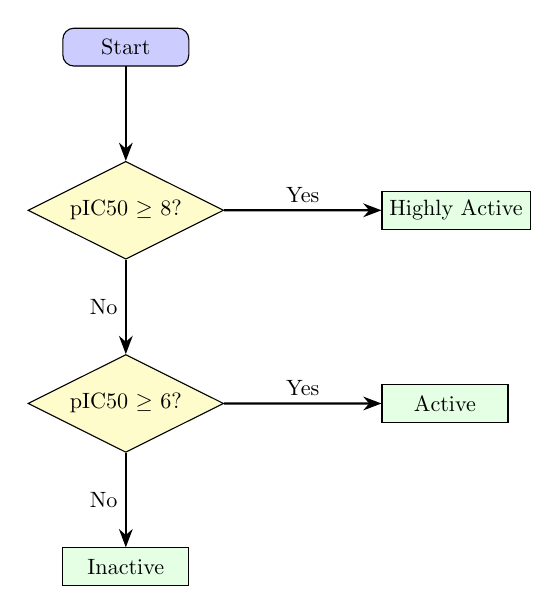
\begin{tikzpicture}[node distance=1.2cm, scale=0.8, every node/.style={scale=0.8}]
            \node (start) [startstop] {Start};
            \node (cond1) [decision, below=of start] {pIC50 $\geq$ 8?};
            \node (active) [process, right=2cm of cond1] {Highly Active};
            \node (cond2) [decision, below=of cond1] {pIC50 $\geq$ 6?};
            \node (moderate) [process, right=2cm of cond2] {Active};
            \node (inactive) [process, below=of cond2] {Inactive};
            
            \draw[arrow] (start) -- (cond1);
            \draw[arrow] (cond1) -- node[above] {Yes} (active);
            \draw[arrow] (cond1) -- node[left] {No} (cond2);
            \draw[arrow] (cond2) -- node[above] {Yes} (moderate);
            \draw[arrow] (cond2) -- node[left] {No} (inactive);
        \end{tikzpicture}
    \end{center}
\end{frame}

\begin{frame}[fragile]{Lesson 4 Code Example}
    \small
    \begin{lstlisting}[style=codeStyle]
# Classify compound activity by pIC50
pic50 = 7.5
if pic50 >= 8:
    activity = "Highly Active"
elif pic50 >= 6:
    activity = "Active"
elif pic50 >= 5:
    activity = "Moderate"
else:
    activity = "Inactive"
print(f"pIC50 {pic50}: {activity}")

# Codon identification (Python 3.10+)
codon = "ATG"
match codon:
    case "ATG":
        print("Start codon (Methionine)")
    case "TAA" | "TAG" | "TGA":
        print("Stop codon")
    case _:
        print("Coding codon")
    \end{lstlisting}
\end{frame}

% --- LAB 4 ---
\begin{frame}{\textcolor{labcolor}{Lab 4: Conditionals}}
    \small
    \textbf{Objective:} Implement decision logic for compound classification.
    \vspace{0.5em}
    \begin{block}{Exercise 4.1 -- Drug-Likeness Checker}
        Create a program that checks Lipinski Rule of Five:\\
        Input: MW, LogP, HBD, HBA\\
        Output: Number of violations (0--4)\\
        Print ``Drug-like'' if violations $\leq$ 1, else ``Non-drug-like''
    \end{block}
    \vspace{0.5em}
    \begin{block}{Exercise 4.2 -- Codon Identifier}
        Given a 3-letter codon, identify if it's:
        \begin{itemize}
            \item Start codon: ``ATG''
            \item Stop codon: ``TAA'', ``TAG'', ``TGA''
            \item Other: any other codon
        \end{itemize}
    \end{block}
\end{frame}

\begin{frame}{\textcolor{labcolor}{Lab 4: Conditionals (cont.)}}
    \footnotesize
    \begin{block}{Exercise 4.3 -- Activity Classifier}
        Classify compound based on pIC50:
        \begin{itemize}\setlength{\itemsep}{0pt}
            \item pIC50 $\geq$ 8: ``Highly Active''
            \item 7 $\leq$ pIC50 $<$ 8: ``Active''
            \item 6 $\leq$ pIC50 $<$ 7: ``Moderately Active''
            \item 5 $\leq$ pIC50 $<$ 6: ``Weakly Active''
            \item pIC50 $<$ 5: ``Inactive''
        \end{itemize}
        Test with values: 8.5, 7.2, 6.5, 5.3, 4.1
    \end{block}
\end{frame}

% ============================================
% LESSON 5: LOOPS
% ============================================
\subsection{Lesson 5: Loops}

\begin{frame}{Lesson 5: Learning Objectives}
    \small
    \textbf{Learning Objectives:}
    \begin{itemize}
        \item Iterate over sequences using for loops
        \item Use while loops for conditional repetition
        \item Control loop flow with break and continue
    \end{itemize}
    \vspace{0.5em}
    \textbf{Applications:}
    \begin{itemize}
        \item Process compound libraries (batch MW calculation)
        \item Count nucleotide frequencies (Rosalind DNA)
        \item Screen compounds against activity thresholds
    \end{itemize}
\end{frame}

\begin{frame}{Lesson 5: Loops}
    \small
    \texttt{for} loop: iterate sequences/range\\
    \texttt{while} loop: repeat until condition False\\
    \texttt{break}/\texttt{continue}: control loop flow
    \vspace{0.5em}
    \begin{center}
        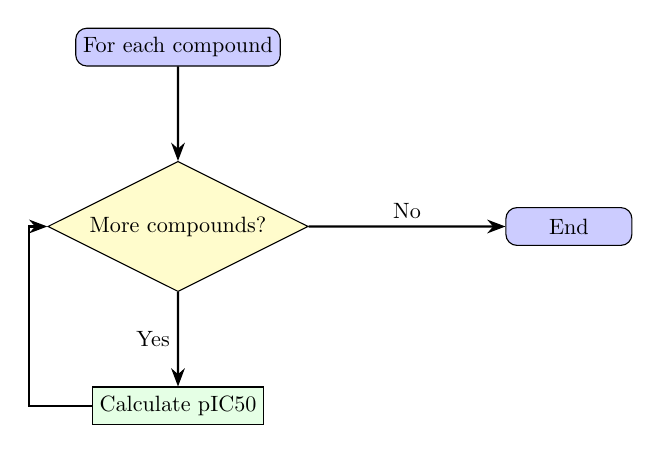
\begin{tikzpicture}[node distance=1.2cm, scale=0.8, every node/.style={scale=0.8}]
            \node (start) [startstop] {For each compound};
            \node (cond) [decision, below=of start] {More compounds?};
            \node (body) [process, below=of cond] {Calculate pIC50};
            \node (end) [startstop, right=2.5cm of cond] {End};
            
            \draw[arrow] (start) -- (cond);
            \draw[arrow] (cond) -- node[above] {No} (end);
            \draw[arrow] (cond) -- node[left] {Yes} (body);
            \draw[arrow] (body.west) -- ++(-1,0) |- (cond.west);
        \end{tikzpicture}
    \end{center}
\end{frame}

\begin{frame}[fragile]{Lesson 5 Code Example: For Loops}
    \small
    \begin{lstlisting}[style=codeStyle]
import math

# Process compound library - calculate pIC50
ic50_values = [5.2, 120.0, 8.7, 2.1, 450.0]  # nM
for ic50 in ic50_values:
    pic50 = 9 - math.log10(ic50)
    print(f"IC50: {ic50:>6.1f} nM -> pIC50: {pic50:.2f}")

# Count nucleotides in DNA sequence
dna = "ATGCGATCGATCG"
counts = {"A": 0, "T": 0, "G": 0, "C": 0}
for nucleotide in dna:
    counts[nucleotide] += 1
print(f"Nucleotide counts: {counts}")

# Find active compounds (break/continue)
compounds = [("CPD1", 7.2), ("CPD2", 5.1), ("CPD3", 8.5)]
for name, pic50 in compounds:
    if pic50 < 6: continue  # skip inactive
    print(f"{name}: Active (pIC50={pic50})")
    \end{lstlisting}
\end{frame}

\begin{frame}[fragile]{Lesson 5 Code Example: While Loops}
    \small
    \begin{lstlisting}[style=codeStyle]
# While loop: find first potent compound (pIC50 >= 7.5)
pic50_values = [5.2, 5.8, 6.1, 7.5, 8.2, 6.8]
i = 0
while i < len(pic50_values):
    if pic50_values[i] >= 7.5:
        print(f"First potent at index {i}: pIC50={pic50_values[i]}")
        break  # exit loop when found
    i += 1

# While loop with user input simulation
threshold = 6.0
compound_count = 0
max_compounds = 5
while compound_count < max_compounds:
    # Simulate reading compounds until reaching limit
    compound_count += 1
    print(f"Processing compound {compound_count}")

# While with sentinel value
sequence = ""
codons = ["ATG", "CGA", "TCG", "TAA"]  # TAA is stop
idx = 0
while idx < len(codons) and codons[idx] != "TAA":
    sequence += codons[idx]
    idx += 1
print(f"Sequence before stop: {sequence}")  # ATGCGATCG
    \end{lstlisting}
\end{frame}

% --- LAB 5 ---
\begin{frame}{\textcolor{labcolor}{Lab 5: Loops}}
    \footnotesize
    \textbf{Objective:} Process collections of compounds and sequences.
    \vspace{0.3em}
    \begin{block}{Exercise 5.1 -- Batch IC50 Conversion}
        Convert list of IC50 values (nM) to pIC50:\\
        IC50\_list = [1.0, 10.0, 100.0, 1000.0, 10000.0]\\
        Use a for loop to calculate and print each pIC50.
    \end{block}
    \vspace{0.2em}
    \begin{block}{Exercise 5.2 -- Nucleotide Counter (Rosalind DNA)}
        Count all nucleotides in a DNA sequence using a for loop:\\
        seq = ``AGCTTTTCATTCTGACTGCAACGGGCAATATGTCTCTGTGT''\\
        Print counts for A, C, G, T separated by spaces.
    \end{block}
\end{frame}

\begin{frame}{\textcolor{labcolor}{Lab 5: Loops (cont.)}}
    \footnotesize
    \begin{block}{Exercise 5.3 -- Filter Active Compounds}
        Given pIC50 values: [5.2, 6.8, 7.3, 4.9, 8.1, 5.9, 6.2]\\
        Use a for loop with continue to skip inactive (pIC50 $<$ 6). Print only active compounds.
    \end{block}
    \vspace{0.2em}
    \begin{block}{Exercise 5.4 -- Find First Potent (While Loop)}
        Given pIC50 values: [5.2, 5.8, 6.1, 7.5, 8.2, 6.8]\\
        Use a while loop with break to find the first ``highly potent'' compound (pIC50 $\geq$ 7.5). Print its index and value.\\
        \textit{Hint: Use index variable i, increment i += 1, check condition before break.}
    \end{block}
\end{frame}

\begin{frame}{\textcolor{labcolor}{Lab 5: Loops (cont.)}}
    \footnotesize
    \begin{block}{Exercise 5.5 -- Read Until Stop Codon (While Loop)}
        Given codons: [``ATG'', ``CGA'', ``TCG'', ``GGC'', ``TAA'', ``AAA'']\\
        Use a while loop to read codons and build a sequence string.\\
        Stop when you encounter a stop codon (``TAA'', ``TAG'', or ``TGA'').\\
        Print the sequence built before the stop codon.
    \end{block}
    \vspace{0.2em}
    \begin{block}{Exercise 5.6 -- Compound Screening (While Loop)}
        Simulate screening compounds until finding 3 active ones:\\
        Given: [4.5, 5.2, 6.8, 5.1, 7.3, 4.9, 8.1, 5.9]\\
        Use while loop, count actives (pIC50 $\geq$ 6), stop when count reaches 3.\\
        Print how many compounds were screened.
    \end{block}
\end{frame}

% ============================================
% LESSON 6: FUNCTIONS
% ============================================
\subsection{Lesson 6: Functions}

\begin{frame}{Lesson 6: Learning Objectives}
    \small
    \textbf{Learning Objectives:}
    \begin{itemize}
        \item Define reusable functions with parameters
        \item Use return statements to output results
        \item Apply *args and **kwargs for flexible inputs
    \end{itemize}
    \vspace{0.5em}
    \textbf{Applications:}
    \begin{itemize}
        \item Create IC50 $\to$ pIC50 converters
        \item Build Lipinski property calculators
        \item Implement sequence analysis functions (GC, REVC)
    \end{itemize}
\end{frame}

\begin{frame}{Lesson 6: Functions}
    \small
    \texttt{def name(params):} define function\\
    \texttt{return} for return value\\[0.3em]
    \textbf{Special Parameters:}
    \begin{itemize}
        \item \texttt{*args} -- accepts any number of \textbf{positional} arguments as a tuple
        \item \texttt{**kwargs} -- accepts any number of \textbf{keyword} arguments as a dictionary
    \end{itemize}
\end{frame}

\begin{frame}[fragile]{Lesson 6 Code Example: Basic Functions}
    \small
    \begin{lstlisting}[style=codeStyle]
import math

# Function: IC50 to pIC50 conversion
def ic50_to_pic50(ic50_nm):
    """Convert IC50 (nM) to pIC50."""
    return -math.log10(ic50_nm * 1e-9)

# Function with validation (returns tuple)
def calculate_mw(smiles):
    """Calculate MW from SMILES using RDKit."""
    from rdkit import Chem
    from rdkit.Chem import Descriptors
    mol = Chem.MolFromSmiles(smiles)
    if mol is None:
        return None, "Invalid SMILES"
    return Descriptors.MolWt(mol), "Success"

# Usage
print(ic50_to_pic50(10))  # 8.0
mw, status = calculate_mw("CCO")
print(f"MW: {mw:.2f}, Status: {status}")
    \end{lstlisting}
\end{frame}

\begin{frame}[fragile]{Lesson 6 Code Example: *args and **kwargs}
    \small
    \begin{lstlisting}[style=codeStyle]
# *args - accept variable number of positional arguments
def average_activity(*pic50_values):
    """Calculate average pIC50 from multiple values."""
    return sum(pic50_values) / len(pic50_values)

# **kwargs - accept variable number of keyword arguments
def print_compound(**props):
    """Print compound properties as key-value pairs."""
    for key, value in props.items():
        print(f"{key}: {value}")

# Usage examples
avg = average_activity(5.2, 6.8, 7.3, 8.1)
print(f"Average pIC50: {avg:.2f}")

print_compound(name="Aspirin", MW=180.16, pIC50=5.2)
    \end{lstlisting}
\end{frame}

% --- LAB 6 ---
\begin{frame}{\textcolor{labcolor}{Lab 6: Functions}}
    \footnotesize
    \textbf{Objective:} Create reusable molecular utility functions.
    \vspace{0.2em}
    \begin{block}{Exercise 6.1 -- pIC50 Converter Function}
        Create function: \texttt{ic50\_to\_pic50(ic50\_nm)}\\
        Input: IC50 in nanomolar. Output: pIC50 value.\\
        Test with: 10, 100, 1000 nM
    \end{block}
    \vspace{0.2em}
    \begin{block}{Exercise 6.2 -- GC Content Function}
        Create function: \texttt{gc\_content(sequence)}\\
        Input: DNA sequence string. Output: GC percentage (float).\\
        Test with: ``AGCTATAG'', ``GCGCGCGC'', ``ATATAT''
    \end{block}
\end{frame}

\begin{frame}{\textcolor{labcolor}{Lab 6: Functions (cont.)}}
    \footnotesize
    \begin{block}{Exercise 6.3 -- Lipinski Calculator}
        Create function: \texttt{check\_lipinski(mw, logp, hbd, hba)}\\
        Returns tuple: (passes: bool, violations: int). Test with multiple compound property sets.
    \end{block}
    \vspace{0.2em}
    \begin{block}{Exercise 6.4 -- Reverse Complement Function}
        Create function: \texttt{reverse\_complement(dna)}\\
        Input: DNA sequence. Output: Reverse complement sequence.\\
        Test with Rosalind REVC sample: ``AAAACCCGGT'' $\to$ ``ACCGGGTTTT''
    \end{block}
\end{frame}

% ============================================
% LESSON 6B: ERROR HANDLING
% ============================================
\subsection{Lesson 6B: Error Handling}

\begin{frame}{Lesson 6B: Learning Objectives}
    \small
    \textbf{Learning Objectives:}
    \begin{itemize}
        \item Handle runtime errors with try/except blocks
        \item Use else and finally for cleanup operations
        \item Raise custom exceptions for validation
    \end{itemize}
    \vspace{0.5em}
    \textbf{Applications:}
    \begin{itemize}
        \item Handle invalid SMILES parsing gracefully
        \item Manage missing data in compound datasets
        \item Validate FASTA file formats
    \end{itemize}
\end{frame}

\begin{frame}{Lesson 6B: Error Handling (try/except)}
    \small
    \textbf{Concept:} Handle runtime errors gracefully\\[0.5em]
    \textbf{Keywords:} \texttt{try}, \texttt{except}, \texttt{else}, \texttt{finally}, \texttt{raise}\\[0.5em]
    \textbf{Common Exceptions:}
    \begin{itemize}
        \item \texttt{ValueError} -- invalid value conversion
        \item \texttt{TypeError} -- wrong type operation
        \item \texttt{ZeroDivisionError} -- division by zero
        \item \texttt{FileNotFoundError} -- file doesn't exist
        \item \texttt{KeyError} -- dict key not found
    \end{itemize}
\end{frame}

\begin{frame}[fragile]{Lesson 6B Code Example}
    \small
    \begin{lstlisting}[style=codeStyle]
# Basic try/except
try:
    num = int(input("Enter number: "))
    result = 10 / num
except ValueError:
    print("Invalid input!")
except ZeroDivisionError:
    print("Cannot divide by zero!")
else:
    print(f"Result: {result}")
finally:
    print("Execution complete")

# Raising exceptions
def divide(a, b):
    if b == 0:
        raise ValueError("Divisor cannot be zero")
    return a / b
    \end{lstlisting}
\end{frame}

% --- LAB 6B ---
\begin{frame}{\textcolor{labcolor}{Lab 6B: Error Handling}}
    \footnotesize
    \textbf{Objective:} Build robust code that handles invalid inputs.
    \vspace{0.2em}
    \begin{block}{Exercise 6B.1 -- Safe IC50 Conversion}
        Modify \texttt{ic50\_to\_pic50()} to handle: Negative IC50 values (raise ValueError), Zero IC50 (raise ValueError), Non-numeric input (catch TypeError).\\
        Return None on error and print helpful message.
    \end{block}
    \vspace{0.2em}
    \begin{block}{Exercise 6B.2 -- SMILES Validator}
        Create function that validates SMILES:\\
        Use RDKit: \texttt{Chem.MolFromSmiles(smiles)}\\
        If returns None, raise ValueError with message.\\
        Handle with try/except and return valid/invalid status.
    \end{block}
\end{frame}

% ============================================
% SECTION 2: COLLECTIONS
% ============================================
\section{Collections \& Advanced Python (Lessons 7--12)}

% ============================================
% LESSON 7: LISTS
% ============================================
\subsection{Lesson 7: Lists}

\begin{frame}{Lesson 7: Learning Objectives}
    \small
    \textbf{Learning Objectives:}
    \begin{itemize}
        \item Create and modify lists using built-in methods
        \item Access elements via indexing and slicing
        \item Perform common list operations (append, remove, sort)
    \end{itemize}
    \vspace{0.5em}
    \textbf{Applications:}
    \begin{itemize}
        \item Store SMILES strings for compound libraries
        \item Manage pIC50 activity measurements
        \item Build queues for batch processing
    \end{itemize}
\end{frame}

\begin{frame}{Lesson 7: Python Lists}
    \small
    Lists store ordered sequences.\\[0.5em]
    \textbf{Methods:} \texttt{append}, \texttt{extend}, \texttt{insert}, \texttt{remove}, \texttt{pop}, \texttt{clear}, \texttt{index}, \texttt{count}, \texttt{copy}\\[0.5em]
    \textbf{Scenarios:} SMILES list, pIC50 values, compound IDs
\end{frame}

\begin{frame}[fragile]{Lesson 7 Code Example}
    \small
    \begin{lstlisting}[style=codeStyle]
smiles_list = ["CCO", "CC(=O)O", "c1ccccc1"]
smiles_list.append("CCN")
smiles_list.insert(1, "CC")
smiles_list.remove("CCO")
print(smiles_list[0], smiles_list[-1])

# pIC50 statistics
pic50_values = [5.2, 6.8, 7.3, 4.9, 8.1]
print(f"Min: {min(pic50_values)}")
print(f"Max: {max(pic50_values)}")
print(f"Sorted: {sorted(pic50_values)}")
    \end{lstlisting}
\end{frame}

% --- LAB 7 ---
\begin{frame}{\textcolor{labcolor}{Lab 7: Lists}}
    \footnotesize
    \textbf{Objective:} Manage compound libraries using lists.
    \vspace{0.2em}
    \begin{block}{Exercise 7.1 -- Compound Library}
        Create a list of SMILES strings for 5 common drugs.\\
        Perform operations:
        \begin{itemize}\setlength{\itemsep}{0pt}
            \item Add a new compound
            \item Remove a compound by value
            \item Insert at specific position
            \item Print first and last compounds
        \end{itemize}
    \end{block}
    \vspace{0.2em}
    \begin{block}{Exercise 7.2 -- pIC50 Statistics}
        Given: [5.2, 6.8, 7.3, 4.9, 8.1, 5.9, 6.2, 7.8]\\
        Calculate: min, max, sorted list, count of actives ($\geq$6)
    \end{block}
\end{frame}

% ============================================
% LESSON 7B: TUPLES & SETS
% ============================================
\subsection{Lesson 7B: Tuples \& Sets}

\begin{frame}{Lesson 7B: Learning Objectives}
    \small
    \textbf{Learning Objectives:}
    \begin{itemize}
        \item Use tuples for immutable data records
        \item Apply sets for unique element collections
        \item Perform set operations (union, intersection, difference)
    \end{itemize}
    \vspace{0.5em}
    \textbf{Applications:}
    \begin{itemize}
        \item Store compound records (name, SMILES, pIC50)
        \item Find unique molecular scaffolds
        \item Compare compound libraries
    \end{itemize}
\end{frame}

\begin{frame}[fragile]{Lesson 7B Code Example}
    \small
    \begin{lstlisting}[style=codeStyle]
# Tuples - immutable (compound data)
compound = ("Aspirin", "CC(=O)OC1=CC=CC=C1C(=O)O", 180.16)
name, smiles, mw = compound  # unpacking

# Sets - unique scaffolds
scaffolds = {"benzene", "pyridine", "benzene"}  # 2 unique
scaffolds.add("furan")

# Set operations for compound comparison
lib_A = {"CMP001", "CMP002", "CMP003"}
lib_B = {"CMP002", "CMP003", "CMP004"}
print(lib_A | lib_B)  # union: all compounds
print(lib_A & lib_B)  # intersection: common
print(lib_A - lib_B)  # unique to lib_A
    \end{lstlisting}
\end{frame}

% --- LAB 7B ---
\begin{frame}{\textcolor{labcolor}{Lab 7B: Tuples \& Sets}}
    \footnotesize
    \begin{block}{Exercise 7B.1 -- Compound Records}
        Create tuples for 3 compounds: (name, SMILES, pIC50)\\
        Unpack each tuple and print formatted output.\\
        Try to modify a tuple value -- observe the error.
    \end{block}
    \vspace{0.2em}
    \begin{block}{Exercise 7B.2 -- Library Comparison}
        Library A: \{``CMP001'', ``CMP002'', ``CMP003'', ``CMP004''\}\\
        Library B: \{``CMP003'', ``CMP004'', ``CMP005'', ``CMP006''\}\\
        Find:
        \begin{itemize}\setlength{\itemsep}{0pt}
            \item All unique compounds (union)
            \item Common compounds (intersection)
            \item Compounds only in A / only in B
        \end{itemize}
    \end{block}
\end{frame}

% ============================================
% LESSON 8: LIST COMPREHENSIONS
% ============================================
\subsection{Lesson 8: List Comprehensions}

\begin{frame}{Lesson 8: Learning Objectives}
    \small
    \textbf{Learning Objectives:}
    \begin{itemize}
        \item Write concise list comprehensions
        \item Apply map() and filter() for transformations
        \item Combine functional programming techniques
    \end{itemize}
    \vspace{0.5em}
    \textbf{Applications:}
    \begin{itemize}
        \item Filter active compounds (pIC50 $>$ 6)
        \item Batch convert IC50 to pIC50 values
        \item Extract drug-like compounds
    \end{itemize}
\end{frame}

\begin{frame}[fragile]{Lesson 8 Code Example}
    \small
    \begin{lstlisting}[style=codeStyle]
import math
pic50_values = [5.2, 6.8, 7.3, 4.9, 8.1]

# List comprehension: filter active compounds
actives = [p for p in pic50_values if p >= 6.0]

# Lambda + map: convert pIC50 to IC50 (nM)
ic50_nm = list(map(lambda p: 10**(9-p), pic50_values))

# Filter: highly potent (pIC50 > 7)
potent = list(filter(lambda p: p > 7, pic50_values))

print(f"Active: {actives}")
print(f"Potent: {potent}")
    \end{lstlisting}
\end{frame}

% --- LAB 8 ---
\begin{frame}{\textcolor{labcolor}{Lab 8: List Comprehensions}}
    \footnotesize
    \begin{block}{Exercise 8.1 -- Filter Active Compounds}
        Given pIC50 = [5.2, 6.8, 7.3, 4.9, 8.1, 5.9]\\
        Use list comprehension to filter pIC50 $\geq$ 6.0
    \end{block}
    \vspace{0.2em}
    \begin{block}{Exercise 8.2 -- Batch Conversion}
        Convert IC50 list [10, 100, 1000] to pIC50 using:\\
        a) List comprehension\ \ b) map() with lambda
    \end{block}
    \vspace{0.2em}
    \begin{block}{Exercise 8.3 -- Conditional Comprehension}
        Create list of tuples: [(pIC50, ``Active'') if pIC50 $\geq$ 6 else (pIC50, ``Inactive'')]\\
        for values [5.2, 6.8, 7.3, 4.9, 8.1]
    \end{block}
\end{frame}

% ============================================
% LESSON 9: DICTIONARIES
% ============================================
\subsection{Lesson 9: Dictionaries}

\begin{frame}{Lesson 9: Learning Objectives}
    \small
    \textbf{Learning Objectives:}
    \begin{itemize}
        \item Create and manipulate key-value dictionaries
        \item Access, update, and iterate over dict items
        \item Use dict comprehensions for transformations
    \end{itemize}
    \vspace{0.5em}
    \textbf{Applications:}
    \begin{itemize}
        \item Build compound databases (name $\to$ properties)
        \item Create codon translation tables
        \item Store molecular descriptor lookups
    \end{itemize}
\end{frame}

\begin{frame}[fragile]{Lesson 9 Code Example}
    \small
    \begin{lstlisting}[style=codeStyle]
compound_db = {
    "Aspirin": {"SMILES": "CC(=O)OC1=CC=CC=C1C(=O)O", "pIC50": 5.2},
    "Caffeine": {"SMILES": "CN1C=NC2=C1C(=O)N(C(=O)N2C)C", "pIC50": 4.8}
}

# Add new compound
compound_db["Ibuprofen"] = {
    "SMILES": "CC(C)CC1=CC=C(C=C1)C(C)C(=O)O",
    "pIC50": 6.1
}

# Filter actives (dict comprehension)
actives = {k: v for k, v in compound_db.items() if v["pIC50"] >= 5.0}

print(list(actives.keys()))
    \end{lstlisting}
\end{frame}

% --- LAB 9 ---
\begin{frame}{\textcolor{labcolor}{Lab 9: Dictionaries}}
    \footnotesize
    \begin{block}{Exercise 9.1 -- Compound Database}
        Create a dict of compounds with nested properties:\\
        Key: compound name, Value: dict with SMILES, MW, pIC50, is\_active
    \end{block}
    \vspace{0.2em}
    \begin{block}{Exercise 9.2 -- Codon Table (Rosalind)}
        Create a dict mapping codons to amino acids:\\
        ``ATG'' $\to$ ``M'', ``TGG'' $\to$ ``W'', ``TAA'' $\to$ ``Stop''\\
        Use to translate a short sequence.
    \end{block}
    \vspace{0.2em}
    \begin{block}{Exercise 9.3 -- Dict Comprehension}
        Filter the compound database to only active compounds\\
        using dict comprehension: \{k:v for k,v in ... if ...\}
    \end{block}
\end{frame}

% ============================================
% LESSON 10: FILE HANDLING
% ============================================
\subsection{Lesson 10: File Handling}

\begin{frame}{Lesson 10: Learning Objectives}
    \small
    \textbf{Learning Objectives:}
    \begin{itemize}
        \item Read and write text files using open()
        \item Use context managers (with) for safe file handling
        \item Parse structured file formats (CSV, FASTA)
    \end{itemize}
    \vspace{0.5em}
    \textbf{Applications:}
    \begin{itemize}
        \item Read/write compound CSV files
        \item Parse FASTA sequence files
        \item Export filtered results
    \end{itemize}
\end{frame}

\begin{frame}[fragile]{Lesson 10 Code Example}
    \small
    \begin{lstlisting}[style=codeStyle]
# Write compound data to CSV
with open("compounds.csv", "w") as f:
    f.write("name,smiles,pIC50\n")
    f.write("Aspirin,CC(=O)OC1=CC=CC=C1C(=O)O,5.2\n")

# Read FASTA file
with open("sequence.fasta", "r") as f:
    header = f.readline().strip()  # >sequence_id
    sequence = ""
    for line in f:
        sequence += line.strip()

print(f"Header: {header}")
print(f"Sequence length: {len(sequence)}")
    \end{lstlisting}
\end{frame}

% --- LAB 10 ---
\begin{frame}{\textcolor{labcolor}{Lab 10: File Handling}}
    \footnotesize
    \begin{block}{Exercise 10.1 -- Write Compound CSV}
        Create a CSV file with columns: name, SMILES, pIC50\\
        Write data for 5 compounds using \texttt{with open()}.
    \end{block}
    \vspace{0.2em}
    \begin{block}{Exercise 10.2 -- Read FASTA}
        Create a simple FASTA parser: Read file, extract header (lines starting with $>$), concatenate sequence lines, return dict: \{header: sequence\}
    \end{block}
    \vspace{0.2em}
    \begin{block}{Exercise 10.3 -- Filter and Export}
        Read compound CSV, filter active compounds (pIC50 $\geq$ 6)\\
        Write filtered results to new file ``actives.csv''
    \end{block}
\end{frame}

% ============================================
% LESSON 11: NUMPY
% ============================================
\subsection{Lesson 11: NumPy}

\begin{frame}{Lesson 11: Learning Objectives}
    \small
    \textbf{Learning Objectives:}
    \begin{itemize}
        \item Create and manipulate NumPy arrays
        \item Perform vectorized mathematical operations
        \item Use boolean indexing for data filtering
    \end{itemize}
    \vspace{0.5em}
    \textbf{Applications:}
    \begin{itemize}
        \item Store molecular descriptor matrices
        \item Normalize and scale feature data
        \item Compute statistics on activity arrays
    \end{itemize}
\end{frame}

\begin{frame}[fragile]{Lesson 11 Code Example}
    \small
    \begin{lstlisting}[style=codeStyle]
import numpy as np

# Array creation
arr = np.array([[1, 2, 3], [4, 5, 6], [7, 8, 9]])
zeros = np.zeros((2, 3))
seq = np.arange(0, 10, 2)  # [0, 2, 4, 6, 8]

# Properties
print(arr.shape, arr.dtype, arr.ndim)

# Operations
print(arr * 2)           # element-wise multiply
print(arr.sum(axis=0))   # sum per column
print(arr.mean(axis=1))  # mean per row

# Boolean indexing
mask = arr > 5
print(arr[mask])  # [6, 7, 8, 9]
    \end{lstlisting}
\end{frame}

% --- LAB 11 ---
\begin{frame}{\textcolor{labcolor}{Lab 11: NumPy}}
    \footnotesize
    \begin{block}{Exercise 11.1 -- Descriptor Matrix}
        Create a 2D array of molecular descriptors:\\
        Rows = compounds, Columns = [MW, LogP, HBD, HBA]\\
        Calculate mean and std for each descriptor (column).
    \end{block}
    \vspace{0.2em}
    \begin{block}{Exercise 11.2 -- Normalization}
        Normalize descriptor values to 0-1 range: (x - min) / (max - min)\\
        Use vectorized operations (no loops).
    \end{block}
    \vspace{0.2em}
    \begin{block}{Exercise 11.3 -- Boolean Filtering}
        Filter compounds where MW $<$ 500 AND LogP $<$ 5\\
        Use boolean indexing.
    \end{block}
\end{frame}

% ============================================
% LESSON 11B: PANDAS
% ============================================
\subsection{Lesson 11B: Pandas}

\begin{frame}{Lesson 11B: Learning Objectives}
    \small
    \textbf{Learning Objectives:}
    \begin{itemize}
        \item Create Series and DataFrame structures
        \item Filter, group, and aggregate tabular data
        \item Read/write data from CSV files
    \end{itemize}
    \vspace{0.5em}
    \textbf{Applications:}
    \begin{itemize}
        \item Manage compound libraries with properties
        \item Analyze bioactivity data
        \item Merge descriptor and activity datasets
    \end{itemize}
\end{frame}

\begin{frame}[fragile]{Lesson 11B Code Example}
    \small
    \begin{lstlisting}[style=codeStyle]
import pandas as pd

df = pd.DataFrame({
    'Name': ['Aspirin', 'Ibuprofen', 'Caffeine', 'Drug_X'],
    'pIC50': [5.2, 6.1, 4.8, 7.5],
    'MW': [180.16, 206.28, 194.19, 320.5]
})

# Selection & Filtering
actives = df[df['pIC50'] > 6.0]
drug_like = df[df['MW'] < 500]

# Aggregation
print(df['pIC50'].mean())
print(df.describe())

# GroupBy
df['Class'] = df['pIC50'].apply(lambda x: 'Active' if x >= 6 else 'Inactive')
grouped = df.groupby('Class')['MW'].mean()
    \end{lstlisting}
\end{frame}

% --- LAB 11B ---
\begin{frame}{\textcolor{labcolor}{Lab 11B: Pandas}}
    \footnotesize
    \begin{block}{Exercise 11B.1 -- Create Compound DataFrame}
        Create DataFrame with: Name, SMILES, MW, LogP, pIC50\\
        Add 5+ compounds. Add column for activity class.
    \end{block}
    \vspace{0.2em}
    \begin{block}{Exercise 11B.2 -- Data Analysis}
        Calculate: mean pIC50, count by activity class\\
        Filter drug-like compounds (MW $<$ 500, LogP $<$ 5). Sort by pIC50 descending.
    \end{block}
    \vspace{0.2em}
    \begin{block}{Exercise 11B.3 -- GroupBy Analysis}
        Group compounds by activity class\\
        Calculate mean MW and LogP per group. Export results to CSV.
    \end{block}
\end{frame}

% ============================================
% LESSON 12: JSON & REGEX
% ============================================
\subsection{Lesson 12: JSON \& Regex}

\begin{frame}{Lesson 12: Learning Objectives}
    \small
    \textbf{Learning Objectives:}
    \begin{itemize}
        \item Parse and generate JSON data
        \item Write regex patterns for text matching
        \item Extract and validate patterns in sequences
    \end{itemize}
    \vspace{0.5em}
    \textbf{Applications:}
    \begin{itemize}
        \item Query ChEMBL/PubChem REST APIs
        \item Find restriction sites in DNA sequences
        \item Validate SMILES and sequence formats
    \end{itemize}
\end{frame}

\begin{frame}[fragile]{Lesson 12 Code Example}
    \small
    \begin{lstlisting}[style=codeStyle]
import json
import re

# JSON - PubChem-like data
data = '{"name": "Aspirin", "CID": 2244, "MW": 180.16}'
compound = json.loads(data)
print(compound["name"])

# Regex - find DNA motifs
seq = "ATGCGATCGATCG"
matches = re.findall(r"GATC", seq)  # restriction site
print(f"GATC sites: {len(matches)}")

# Find EcoRI sites
seq2 = "ATGAATTCGCGAATTCTA"
for match in re.finditer(r"GAATTC", seq2):
    print(f"EcoRI site at position {match.start()}")
    \end{lstlisting}
\end{frame}

% --- LAB 12 ---
\begin{frame}{\textcolor{labcolor}{Lab 12: JSON \& Regex}}
    \footnotesize
    \begin{block}{Exercise 12.1 -- Parse PubChem JSON}
        Parse JSON compound data:
        \texttt{\{"CID": 2244, "name": "Aspirin", "MW": 180.16\}}\\
        Extract and print each field.
    \end{block}
    \vspace{0.2em}
    \begin{block}{Exercise 12.2 -- Find Restriction Sites}
        Use regex to find all ``GAATTC'' (EcoRI site) in: ``ATGAATTCGCGAATTCTA''\\
        Print positions of each match.
    \end{block}
    \vspace{0.2em}
    \begin{block}{Exercise 12.3 -- SMILES Validation}
        Use regex to check if SMILES contains aromatic ring (lowercase c, n), ring closure (digits), or double bond (=).
    \end{block}
\end{frame}

% ============================================
% ROSALIND CHALLENGES
% ============================================
\section{Rosalind Bioinformatics Challenges}

\begin{frame}{Rosalind Challenges}
    \footnotesize
    \textbf{Complete these Rosalind.info problems:}
    \vspace{0.3em}
    \begin{enumerate}\setlength{\itemsep}{0pt}
        \item \textbf{DNA} -- Counting DNA Nucleotides
        \item \textbf{RNA} -- Transcribing DNA into RNA
        \item \textbf{REVC} -- Complementing a Strand of DNA
        \item \textbf{GC} -- Computing GC Content
        \item \textbf{HAMM} -- Counting Point Mutations
        \item \textbf{PROT} -- Translating RNA into Protein
        \item \textbf{SUBS} -- Finding a Motif in DNA
        \item \textbf{CONS} -- Consensus and Profile
    \end{enumerate}
    \vspace{0.3em}
    \textbf{Submission:} Upload your solutions to GitHub with clear function documentation and test cases.
\end{frame}

% ============================================
% MINI-PROJECT
% ============================================
\section{Cheminformatics Mini-Project}

\begin{frame}{Mini-Project: QSAR Data Prep Pipeline}
    \footnotesize
    \textbf{Objective:} Build a complete data preparation pipeline.
    \vspace{0.3em}
    \textbf{Tasks:}
    \begin{enumerate}\setlength{\itemsep}{0pt}
        \item Read compound CSV with SMILES and IC50 values
        \item Validate all SMILES using RDKit
        \item Convert IC50 (nM) to pIC50
        \item Calculate Lipinski descriptors (MW, LogP, HBD, HBA)
        \item Add activity class column (Active/Inactive)
        \item Filter drug-like compounds
        \item Export clean dataset to CSV
        \item Generate summary statistics
    \end{enumerate}
    \vspace{0.2em}
    \textbf{Deliverables:} Python script, output CSV, summary report
\end{frame}

% ============================================
% SUMMARY
% ============================================
\section{Summary}

\begin{frame}{Course Summary}
    \footnotesize
    \textbf{Section 1: Python Basics (Lessons 1--6B)}
    \begin{itemize}\setlength{\itemsep}{0pt}
        \item Variables, Data Types, Operators
        \item Strings (SMILES, DNA sequences)
        \item Conditionals and Loops
        \item Functions and Error Handling
    \end{itemize}
    \vspace{0.3em}
    \textbf{Section 2: Collections (Lessons 7--12)}
    \begin{itemize}\setlength{\itemsep}{0pt}
        \item Lists, Tuples, Sets, Dictionaries
        \item List Comprehensions, Lambda Functions
        \item File Handling (CSV, FASTA)
        \item NumPy, Pandas
        \item JSON, Regex
    \end{itemize}
    \vspace{0.3em}
    \textbf{Practice:} Rosalind challenges + QSAR mini-project
\end{frame}

\begin{frame}{Next Steps}
    \footnotesize
    \textbf{Practice Resources:}
    \begin{itemize}\setlength{\itemsep}{0pt}
        \item Rosalind.info for bioinformatics problems
        \item ChEMBL/PubChem for real compound data
        \item RDKit tutorials for cheminformatics
    \end{itemize}
    \vspace{0.3em}
    \textbf{Topics to Explore Next:}
    \begin{itemize}\setlength{\itemsep}{0pt}
        \item Object-Oriented Programming
        \item Machine Learning (scikit-learn)
        \item QSAR/QSPR modeling
        \item Molecular visualization
        \item Deep learning with molecular graphs
    \end{itemize}
    \vspace{0.5em}
    \centering
    \textbf{\Large Good luck with your exercises!}
\end{frame}

\end{document}
